\newpage
\subsection{Lineare Funktionen}

Die Grundform einer jeden linearen Funktion ist $y=k*x+d$.
Wobei...

\begin{itemize}
    \item ... $y$ das das Resultat der Gleichung ist
    \item ... $k$ die Steigung der linearen Funktion ist
    \item ... $x$ die Variable ist
    \item ... $d$ der Abstand zur $x$ Achse ist
\end{itemize}

\hfill \break
Wenn das $k$ der Gleichung...
\begin{itemize}
    \item $>0$ ist wird die Gerade steigend z.B. \textcolor{red}{$y=3x+1$}
    \item $<0$ ist wird die Gerade fallend z.B. \textcolor{green}{$y=-3x+1$}
    \item $=0$ ist wird die Gerade waagrecht z.B. \textcolor{blue}{$y=1$}
\end{itemize}

\hfill \break
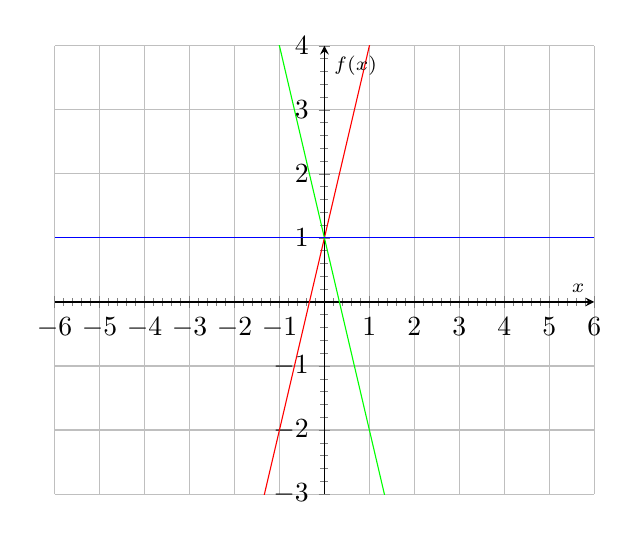
\begin{tikzpicture}[scale=1.0]
    \begin{axis}%
        [
            grid=major,
            xtick={-7,-6,...,7},
            minor x tick num=4, % 4 minor ticks => 5 subintervals
            xmin=-6,
            xmax=6,
            xlabel={\scriptsize $x$},
            axis x line=middle,
            ytick={-5,-4,...,5},
            minor y tick num=4,  % 4 minor ticks => 5 subintervals
            ymin=-3,
            ymax=4,
            ylabel={\scriptsize $f(x)$},
            axis y line=middle,
            no markers,
            samples=100,
            domain=-6:6,
        ]
        \addplot[red] (x,{3*x+1});
        \addplot[green] (x,{-3*x+1});
        \addplot[blue] (x,{1});
    \end{axis}
\end{tikzpicture}